\documentclass[a4paper,UTF8]{article}
\usepackage{ctex}
\usepackage[margin=1.25in]{geometry}
\usepackage{color}
\usepackage{graphicx}
\usepackage{amssymb}
\usepackage{amsmath}
\usepackage{amsthm}
%\usepackage[thmmarks, amsmath, thref]{ntheorem}
\theoremstyle{definition}
\newtheorem*{solution}{Solution}
\newtheorem*{prove}{Proof}
\usepackage{multirow}
\usepackage{url}
\usepackage{enumerate}
\usepackage{algorithm}
\usepackage{algorithmic}
\renewcommand{\algorithmicrequire}{\textbf{Input:}}
\renewcommand{\algorithmicensure}{\textbf{Procedure:}}
\renewcommand\refname{参考文献}

%--

%--
\begin{document}
\title{ POStag}
\author{MG1733099,周天烁,\url{tianshuo.zhou@smail.nju.edu.cn}}
\maketitle

\section*{OverView}
    part-of-speech tagging (POS tagging or PoS tagging or POST)即词性标注是自然语言处理(NLP)中的重要任务之一。具体就是给定由单词序列构成的句子,设计程序自动将单词的词性识别。这里利用隐马尔可夫模型,把词性作为隐状态空间,单词作为观测状态,模型参数$\lambda$=[A,B,π]利用最大似然估计求出,然后利用实验一的维特比算法计算给定句子的最可能的词性序列序列。具体实现如下。
	
	
\section*{Part1.标注预料}
	使用 python自然语言处理工具包nltk的brown语料。该语料的大约有5万个英文句子,其中的每个单词在句子中的词性都已由人工标注,在质量较高,此处想选择的标记符号为最简化的版本,如图1所示。
    \begin{figure}
      \centering
      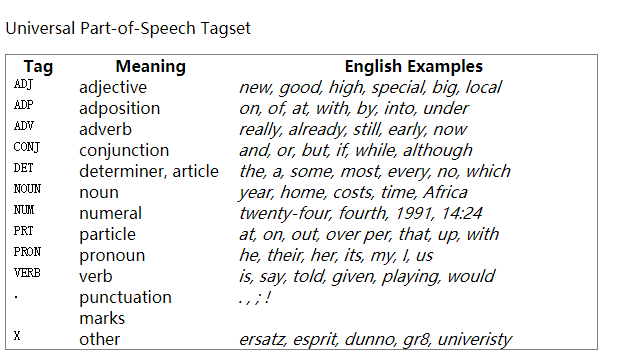
\includegraphics[width=13cm]{1.png}
      \caption{Universal Part-of-Speech Tagset}
      \label{fig:1}
    \end{figure}

\section*{Part2.参数估计}
	各转移矩阵的值通过最大似然估计(Maximum Likelihood Estimation)即统计频率得出。具体实现则可以通过直接调用nltk库函数求出。

\section*{Part3.词性预测 }
	估计出参数后,分别构造单词和词性的索引word2index和tag2index,再建立相应的转移矩阵[A,B,π],通过索引把转移矩阵的每个值填充。

\section*{Part4.实验示例 }
    该程序具有良好的用户界面,用户根据命令行提示输入句子,程序返回标注的词性,然后继续提示用户输入句子,输入大写字母E退出。程序运行示例如图2所示。
    \begin{figure}
      \centering
      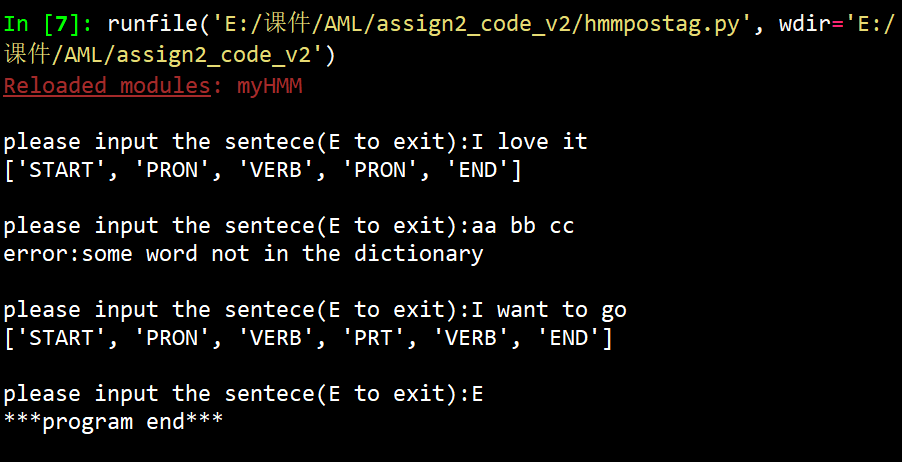
\includegraphics[width=13cm]{2.png}
      \caption{实验示例}
      \label{fig:1}
    \end{figure}
    




\section*{Part5.运行环境 }
    \begin{itemize}
    \item[-]  python3 
    \item[-]  import nltk;import myHMM
    \item[-]  from nltk.corpus import brown(需要下载brown语料库) 
    \end{itemize}

\end{document} 